% !TEX root = ../proposal.tex

\clearpage
\subsection{Consortium as a whole}
\label{sec:consortium}

% The individual members of the consortium are described in a separate
% section 4. There is no need to repeat that information here.

% - Describe the consortium. How will it match the projects objectives?
%   How do the members complement one another (and cover the value
%   chain, where appropriate)? In what way does each of them contribute
%   to the project? How will they be able to work effectively together?
% - If applicable, describe the industrial/commercial involvement in the
%   project to ensure exploitation of the results and explain why this
%   is consistent with and will help to achieve the specific measures
%   which are proposed for exploitation of the results of the project
%   (see section 2.3).
% - Other countries: If one or more of the participants requesting EU
%   funding is based in a country that is not automatically eligible for
%   such funding (entities from Member States of the EU, from Associated
%   Countries and from one of the countries in the exhaustive list
%   included in General Annex A of the work programme are automatically
%   eligible for EU funding), explain why the participation of the
%   entity in question is essential to carrying out the project


\subsubsection{Consortium}
%\label{sec:consortium}

The \Project{} consortium consists of five leading partners which fully cover the entire spectrum of know-how necessary to carry out the planned project.  They belong to the technological leaders in their corresponding domains.

Over the past decade, all partners have continuously developed state-of-the art techniques in various areas of robotics and automated driving and all research partners were consortium members of the EUROPA project. Thus, individual partners cooperated already and between them there are overlapping interests. This guarantees that the
interfaces are well understood and at the same time greatly facilitates the collaboration of the individual partners. The integration of these partners in the \Project{} consortium therefore will lead to a substantial synergy effect that will provide innovative solutions to the problems of robot navigation with incomplete map information, navigation in human-populated environments, online semantic scene interpretation, lifelong operation, map handling, sensor calibration, and interaction between people and the robot as well as with other traffic participants such as cars. The following table summarizes the complementary expertise of the involved partners.
%(see also Figure~\ref{fig:puzzle}):

\begin{center}
\small
  \begin{tabular}[h]{|l|p{14cm}|}\hline
    {\highlightCell Partner} & {\highlightCell Expertise}\\\hline\hline
    \VW  & Assisted and automated driving, navigation, data fusion, environment modeling, system integration\\ \hline
    \ETHZ  & Robotics, autonomous cars, calibration, robot navigation, modeling human behavior, system integration \\ \hline
    \IBM  & Cloud deployment, high performance and cognitive computing, analytics  \\ \hline
    \CLUJ & Perception, stereo-vision based perception, detection, tracking, classification, environment representation, scene understanding\\ \hline
    \PRAGUE & {\cbl Perception, pattern recognition, stereo vision, camera geometry and 3D vision, object tracking, learnable detectors, bayesian modeling} \\ \hline
  \end{tabular}
\end{center}

The coordinator of the project will be \Coordinator{} from Driver Assistance and Integrated Safety Department at Volkswagen Group Research. In the past, \VW{} has successfully participated in
several European projects listed below. Also the other members of the
consortium have a long history of project participation and thus
experience in carrying out European projects, the subsequent table
shows a list of completed and ongoing EU-funded and other relevant projects.

\begin{center}
\begin{tabular}[h]{|l|p{14cm}|}\hline
    {\highlightCell Partner} & {\highlightCell Previous EU-funded projects}\\\hline\hline
    \VW & V-Charge, AdaptIVe, interactIVe, ARTRAC, HAVEit, euroFOT, INTERSAFE-2
    \\ \hline
    \ETHZ & V-Charge, SHERPA, Flourish, TRADR, EUROPA, EUROPA2
    \\ \hline
    \IBM & NANOSTREAMS, EXA2GREEN, TEXT
    \\ \hline
    \CLUJ & R5-COP, PAN-Robots, DRIVE C2X, INSEMTIVES, LarKC, INTERSAFE-2
	\\ \hline
    \PRAGUE & {\cbl TRADR, interactIVe, CloPeMa, NIFTi, PRoViDE, eTRIMS, DIRAC, HUMAVIPS}
    \\ \hline
  \end{tabular}
\end{center}

\clearpage
In the \Project{} project, each partner commits knowledge in their core field of expertise leading to the following assignment of contributions. Note that only the key contributions are listed; for a detailed overview, please consult Section~\ref{sec:workpackages}.
\begin{center}
  \begin{tabular}[h]{|l|p{14cm}|}\hline
    {\highlightCell Partner} & {\highlightCell Key contributions in \Project{}}\\\hline\hline
    \VW & vehicle build-up, data fusion and environment representation, navigation, integration, management of the project
    \\ \hline
    \ETHZ & Accurate all-time metric localization; lifelong large-scale mapping; map management and map summarization.
    \\ \hline
    \IBM & cloud infrastructure; software deployment and test infrastructure; knowledge representation and maintenance; analytics
    \\ \hline
    \CLUJ & 360 degrees redundant perception solution based on available or new 2D and 3D sensors and on the spatio-temporal and appearance based low level representation; Robust algorithms necessary for perception adaptation to adverse visibility conditions, road infrastructure perception, real time 3D terrain perception, road user perception and signaling perception; Object level multi-sensor fusion that allows perception refinement offering an increased robustness and accuracy of the detection, tracking and classification methods.
    \\ \hline
	\PRAGUE & Algorithms for scene understanding, exploiting the perception and data fusion from heterogeneous sensor set, 3D terrain perception
    \\ \hline
 \end{tabular}
\end{center}


\subsubsection{Sub-Contracting}
\label{sec:subcontracting}
Subcontracting will not be used in the project.


\subsubsection{Other Countries}
The Swiss consortium members \ETHZ, and \IBM{} are considered under the category ''industrialised third country'' for Industrial Leadership submissions. As such they do not request funding from the EC (see Figure~\ref{fig:budgetoverview}, on page~\pageref{fig:budgetoverview}). If the proposal is selected, the Swiss members of the \Project{} project will receive funding from the Swiss government directly.



%--------------------------------------------


\subsection{Resources to be committed}
\label{sec:resources}
\subsubsection{Budget overview}
The majority of the requested budget is caused by personnel expenses. The university partners will mainly
employ Ph.D. students and postdocs to carry out the work described above, while the industrial partners employ technical experts and experienced scientists. The detailed personnel cost and claimed person months for Ph.D. students, postdocs, technical experts, and senior personnel is shown in Figure~\ref{fig:budgetoverview}. The
figure shows the budget broken down in detail, including the direct personnel and other direct costs.
Beside the personnel cost, the partners request between \euro30K and \euro48K for travel costs. This includes
travels to different sites, primarily for the four consortium wide integration weeks to carry out test trials and for data collection and mapping, travels to meetings, conference,
as well as partner exchanges.
Furthermore, budget is allocated for equipment/consumables for the partners. The allocated components differ among the
individual partners, as replicating a full car at all partners' sites would be too expensive and is also
not needed to conduct the project. Two automated vehicle platforms and a cloud infrastructure will be needed within \Project{}. One vehicle will
be located at \VW{} at all times, while the other one will be shared among the other partners. The project intends on re-using one of the cars from the V-Charge project and for that one \VW{} only requests funding for extensions and modifications. \IBM requests equipment funding for the cloud infrastructure that will be required for the computation, maintenance and deployment of the lifelong map as well as learning for scene understanding. While both the vehicles as well as the cloud appear on the budget of single partners, these platforms truly enable the project and serve the entire consortium.
 The other partners only allocate resources for equipment in order to build a sensor platform, or for a mockup platform for the individual tasks at the partners' sites in order to conduct their developments. More details can be found below in the individual budgets of the partners.

\begin{figure}[h]
  \caption{Budget overview.}
  \centering
    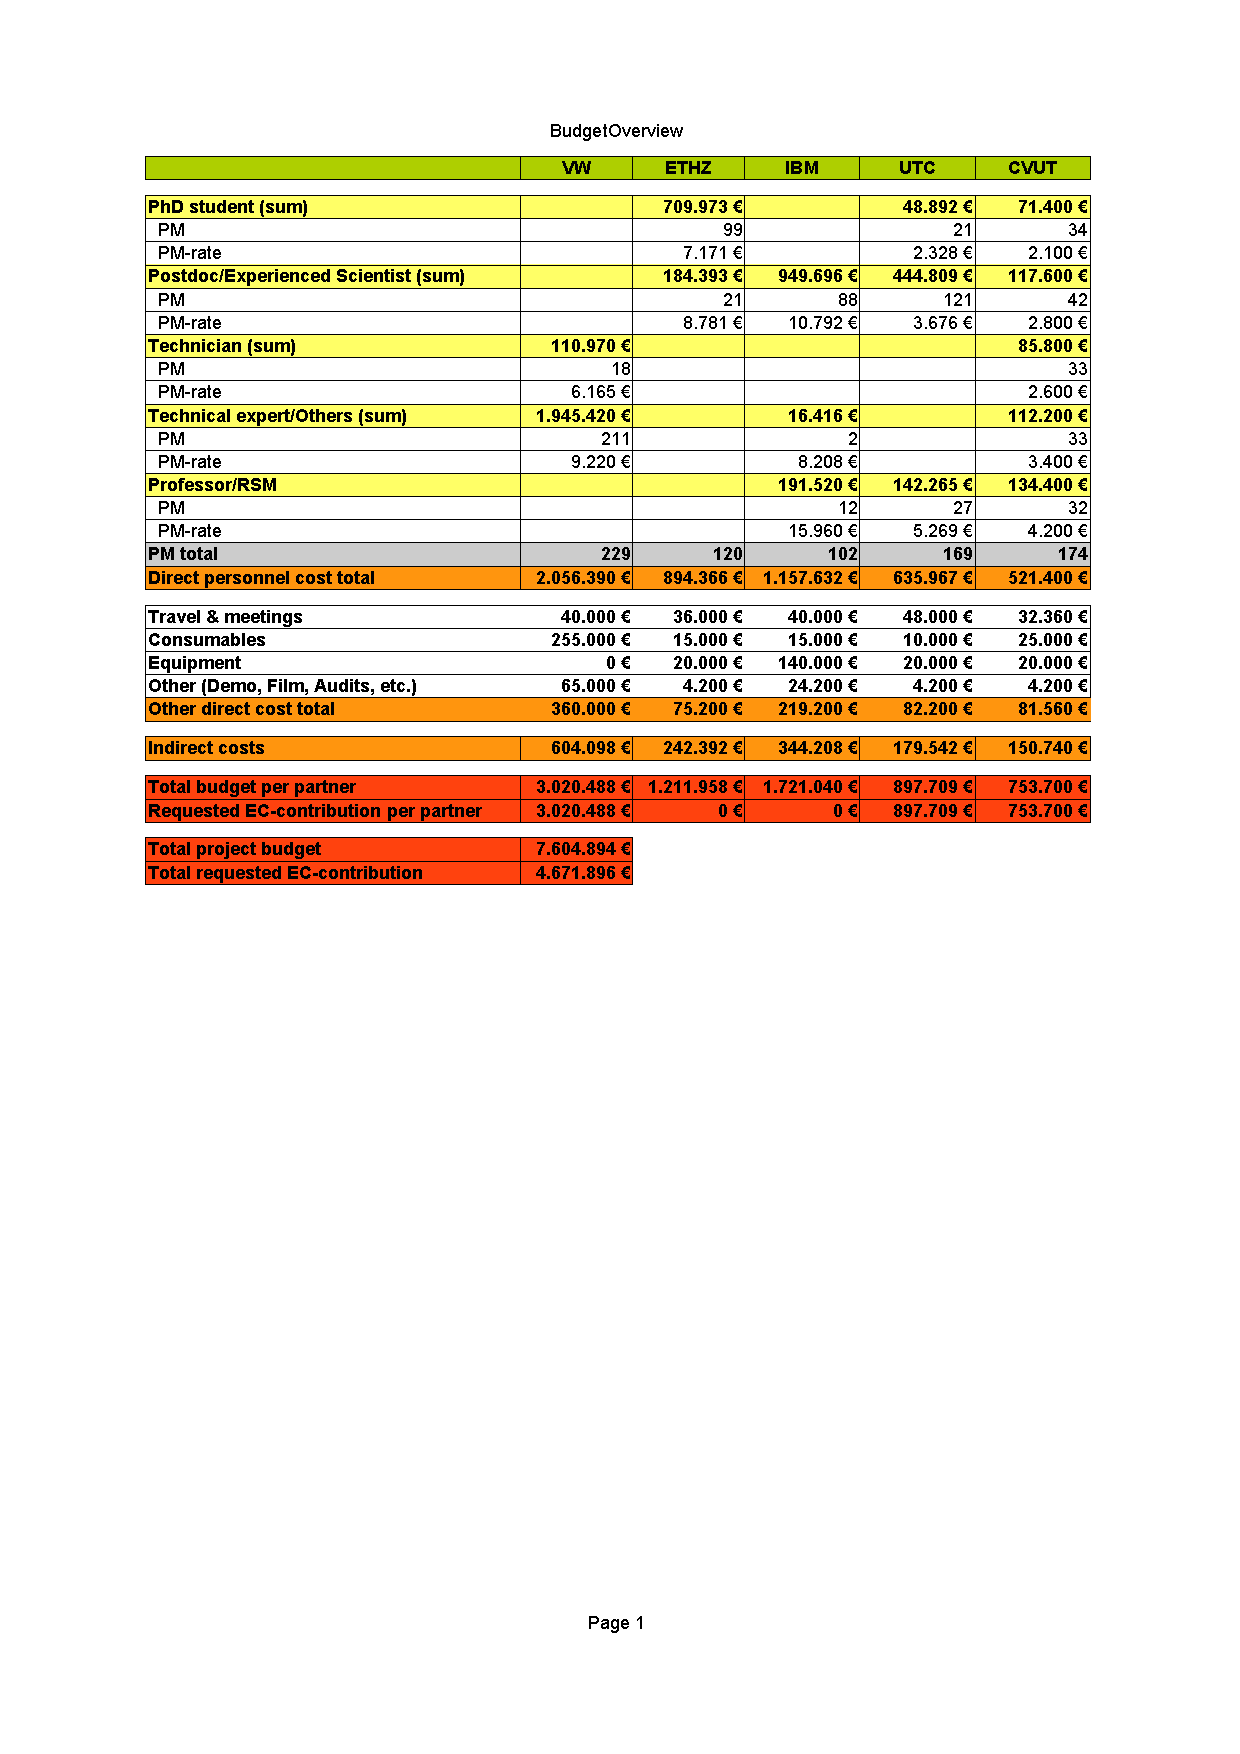
\includegraphics[trim=2cm 13cm 2cm 2.45cm, clip=true, width=0.9\textwidth]{pics/UP-Drive_Budget.pdf}
   \label{fig:budgetoverview}
\end{figure}


\subsubsection{Partner-specific justification for resources}

\ETHZ requests 120 PMs over the project lifetime on RTD activities. This corresponds to 2 Ph.D. students
with 48 and 51 PMs, respectively, and a postdoc with 21 PMs. The Ph.D. students and the postdoc will work
on the localization and mapping framework within the project, with one student focusing on online localization, the other on offline mapping. Both will be involved in the integration and testing efforts. The postdoc will oversee this work and focus on integration, testing,
and dissemination activities. Note that the contribution for \ETHZ (\euro 1,211,958) will be provided by Switzerland so that no EC contribution
is needed for \ETHZ.

\VW will devote 229 PMs over the project lifetime for RTD and management activities. 140 PMs will be split almost evenly between the areas: perception, navigation and integration + the associated tasks of specification and dissemination. This corresponds to 3 technical experts working full-time on their respective fields throughout the project. The adaptation and build-up of the two vehicles will be prepared and validated by an technical expert and performed by technicians, resulting in an effort of 24 and 18 PMs in the respective cost-categories. Additional 22 PMs will be devoted to scene understanding. Project coordination will require 25 PMs. Apart from the personnel costs \VW will also have substantial Consumable costs (\euro 255,000) which will be devoted to equipping the vehicles with sensor systems, computer hardware, safety elements and other items necessary to complete the test and demonstration platforms. Regarding other costs, \VW expects \euro 50,000 costs for the organization of the final demonstration with press representatives as well as further \euro 15,000 for items such as project logo, press materials and audit. In total \VW requests a contribution from the EC of \euro 3,020,487.50. For a tabular view, please consult Figure~\ref{fig:budgetoverview}.

\IBM will devote 88 PMs for an experienced scientist, two PMs for a technical expert and 12 PMs for the principal investigator over the project lifetime on RTD and management activities.
The total PM count for experienced scientists will be divided into three positions. The first one, in conjunction with the technical expert, will be in charge of the hardware and cloud infrastructure buildup. The second one will work on the software deployment functionality and map management. The third one will mainly be involved in scene understanding. The P.I. will guide and manage these roles and conduct research on mapping and scene understanding. He further focuses on integration, testing,
and dissemination activities. \IBM in addition needs \euro 140,000 for cloud infrastructure acquisition forming a crucial part of the project. While forming part of the budget of \IBM, the infrastructure will be extensively used by all project partners for computation, storage and communication activities, particularly lifelong mapping and learning for scene understanding. A further \euro 20,000 are needed to compose a project film for dissemination purposes. For a tabular view, please consult Figure~\ref{fig:budgetoverview}. Note that the contribution for \IBM (\euro 1,721,040) will be provided by Switzerland so that no EC contribution is needed for \IBM.

\CLUJ requests 169 PMs over the project lifetime for RTD activities. This
corresponds to 1 PhD student with 21 PMs, 5 post-doc with approx. 24 PMs
each and 1 professor with 27 PMs. The PhD student and 4 postdocs will
work on requirements, data acquisition and development of perception
algorithms. One postdoc will work on scene understanding tasks. The
professor will supervise all the work and focus on integration,
dissemination and management activities. \CLUJ requests a total contribution from the EC of \euro 897,709.

{\cbl \PRAGUE requests 174 PMs over the project lifetime on RTD and project management activities. PhD students will contribute with 34 PMs; the technician with 33 PMs (he will be stationed about half of his efforts in VW to mediate the integration); two post-docs with 42 PMs (one will deal more with perception and the second with the scene understanding tasks); the senior researchers (technical experts) with 33 PMs (providing key methods for perception, scene understanding and integration), two professors with 32 PMs leading research (R. \v{S}\' ara in perception, V. Hlav\' a\v{c} in scene understanding), integration and public dissemination. \PRAGUE requests a total contribution from the EC of \euro 753,700.} 